\documentclass[a4paper]{article}

\usepackage[french]{babel}
\usepackage[utf8]{inputenc}
\usepackage[T1]{fontenc}
\usepackage[top=3cm, bottom=3cm, left=3cm, right=3cm]{geometry}

\usepackage{listings}
\usepackage{framed}
\usepackage{color}
\usepackage{graphicx}
\usepackage{parskip}
\usepackage{hyperref}
\usepackage{verbatim}
\usepackage{soul}


% FOR COLORS WITH PYTHON CODE

% Default fixed font does not support bold face
\DeclareFixedFont{\ttb}{T1}{txtt}{bx}{n}{10} % for bold
\DeclareFixedFont{\ttm}{T1}{txtt}{m}{n}{10}  % for normal

% Custom colors
\definecolor{deepblue}{rgb}{0,0,0.5}
\definecolor{deepred}{rgb}{0.6,0,0}
\definecolor{deepgreen}{rgb}{0,0.5,0}

\setlength{\parindent}{0ex}

\title{Compte Rendu de TME \\ Apprentissage et Reconnaissance de Forme}
\author{Julien Denes, Michael Trazzi}
\date{Mars 2018}

\begin{document}
\maketitle

\section*{Avant-propos}

L'ensemble du travail présenté dans ce rapport, y compris ce document lui-même, son fichier source LaTeX, les figures et surtout le code sur lequel il repose sont disponible à l'adresse suivante : \href{https://github.com/mtrazzi/arf/}{https://github.com/mtrazzi/arf/}.


%%% BEGIN TME 1 %%%

\section*{TME 1 - Arbres de décision, sélection de modèles}

\subsection*{Quelques expériences préliminaires}

\begin{figure}[ht!]
\begin{center}
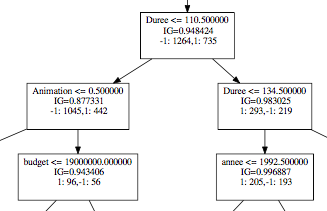
\includegraphics[scale=0.5]{tree5_part}
\caption{une partie de ce qu'on obtient avec profondeur 5}
\label{profondeur}
\end{center}
\end{figure}

Sur les données IMDB, nous avons testé des profondeurs d'arbres allant de 5 à 50. Pour une profondeur de 5 (resp. 50), on obtient un score de 0.736429038587 (resp. 0.900152605189). On observe un \underline{surapprentissage} de nos données dans le cas de la profondeur de 50.  Plus généralement, plus la profondeur est grande, et plus on \underline{surapprend} notre base de données d'apprentissage. Le score ainsi défini \underline{n'est pas un indicateur fiable} : il indique uniquement notre capacité a surapprendre la base d'apprentissage, mais ne tient pas compte du pouvoir de généralisation.

\subsection*{Sur et sous apprentissage}

\begin{figure}[ht!]
\begin{center}
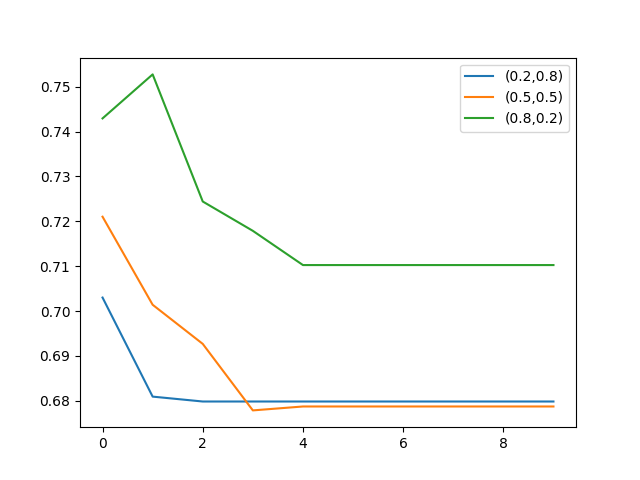
\includegraphics[scale=0.5]{Figure_1}
\caption{Evolution du score en fonction de (profondeur-1)/5 avec toute la base d'apprentissage}
\label{apprentissage_prof1}
\end{center}
\end{figure}

\begin{figure}[ht!]
\begin{center}
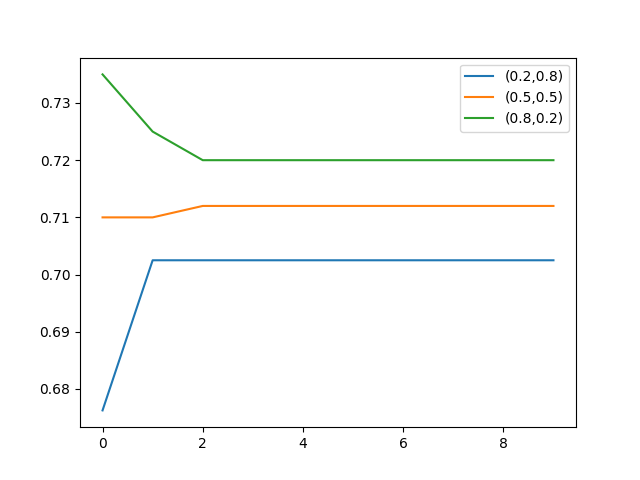
\includegraphics[scale=0.5]{Figure_3}
\caption{Idem avec peu d'exemples (1000 au lieu de 4000)}
\label{apprentissage_prof2}
\end{center}
\end{figure}

Avec peu d'exemples d'apprentissage, \ul{le score se stabilise tres rapidement en fonction de la profondeur}. Avoir un arbre très profond avec seulement 1000 exemples ne fait pas varier le score. A contrario, avec l'ensemble de la base d'apprentissage, \ul{le score continue a varier jusqu'a une prondeur de 25}.

Nos résultats ne nous semblent pas fiables (seulement 5 points pour chaque courbe, base d'apprentissage de seulement quelques milliers d'exemples). Pour les ameéliorer il faudrait prendre \ul{plus d'exemples} (10 000 000), \ul{plus de repartitions} (au moins 5) et \ul{plus de points} (100 profondeurs différentes).


%%% END TME1 %%%

\section*{TME 2 - Estimation de densité - Expérimentations}

Dans cette partie, on cherche à estimer par diverses méthodes la densités de certains Points of Interest (POI) à Paris à partir de données fournis par google maps. Nous avons choisi de travailler avec un POI en particulier: \ul{les nightclubs}.

\begin{figure}[ht!]
\begin{center}
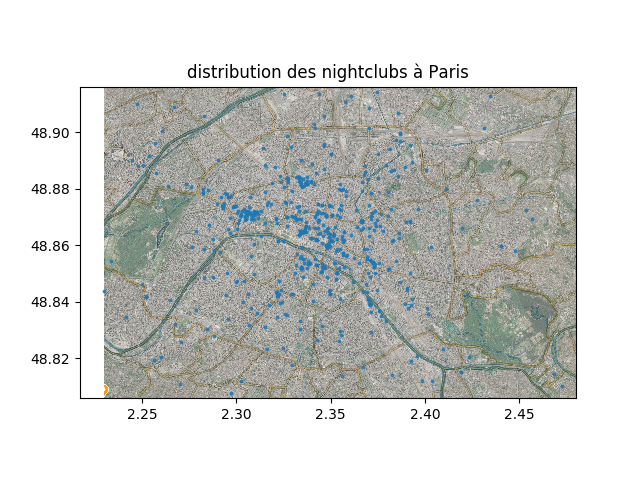
\includegraphics[scale=0.5]{nightclubs.png}
\label{apprentissage_prof2}
\end{center}
\end{figure}

\subsection*{Méthode des histogrammes/noyaux}

Afin d'obtenir une estimation de densité, nous avons utilisé deux méthodes: une méthode par histogramme et une méthode d'estimation par noyaux. Les deux noyaux considérés sont la fenêtre de Parzen et le noyau Gaussien.

\subsection*{Différence entre faible et forte discrétisation}

Pour la méthode des histogrammes nous avons fait varier le pas \verb!h! de discrétisation, inversement proportionnel au nombre de \verb!bins!.

\begin{figure}[ht!]
\begin{center}
\begin{minipage}{0.45\textwidth}
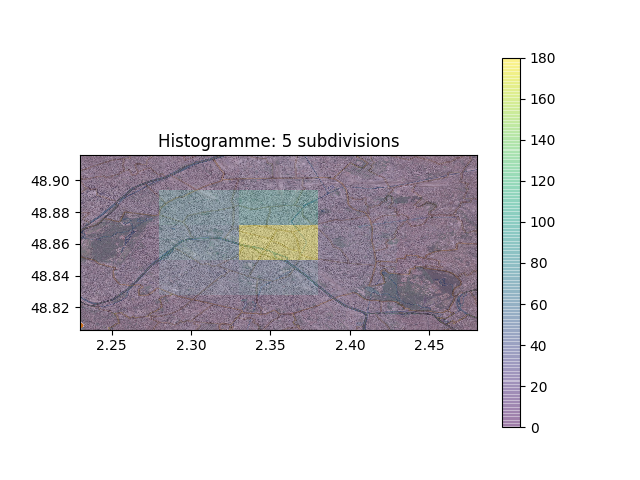
\includegraphics[scale=0.5]{Histo5.png}
\label{f1_trajectoire}
\end{minipage}\hfill
\begin{minipage}{0.45\textwidth}
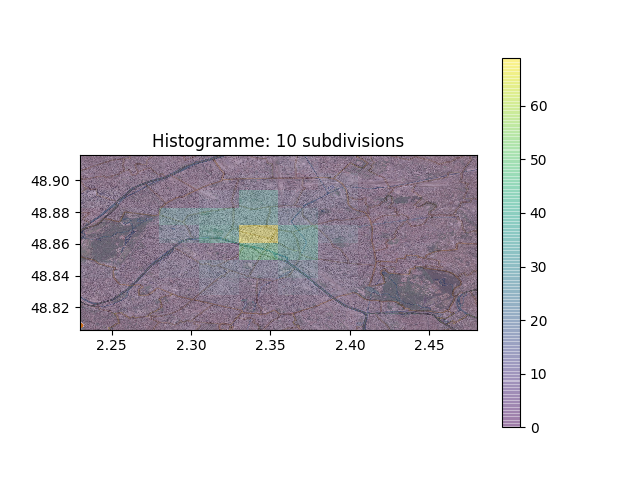
\includegraphics[scale=0.5]{Histo10.png}
\label{f2_trajectoire}
\end{minipage}
\end{center}
\end{figure}

\begin{figure}[ht!]
\begin{center}
\begin{minipage}{0.45\textwidth}
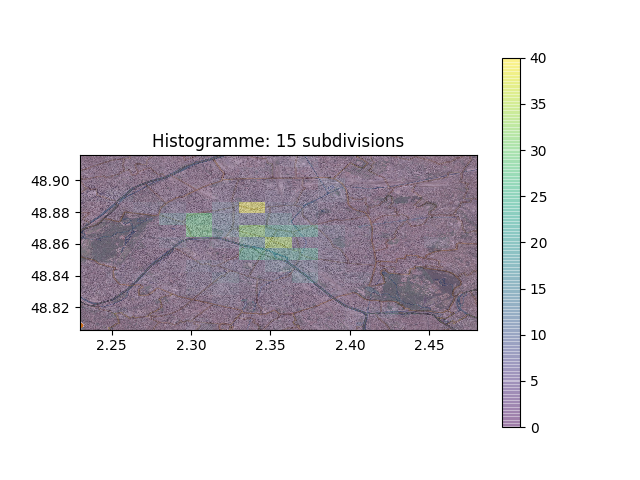
\includegraphics[scale=0.5]{Histo15.png}
\label{f1_trajectoire}
\end{minipage}\hfill
\begin{minipage}{0.45\textwidth}
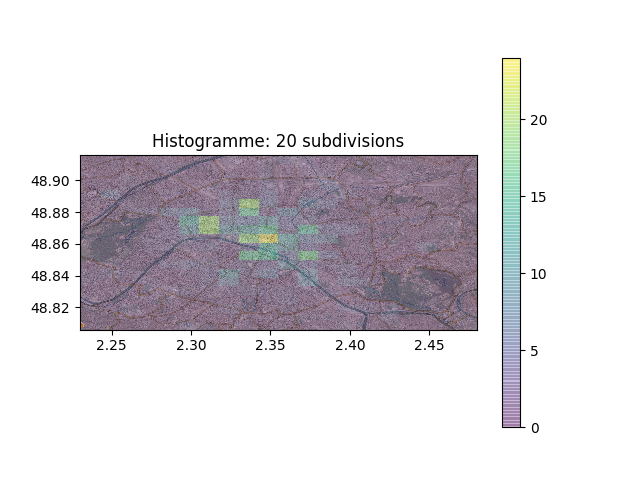
\includegraphics[scale=0.5]{Histo20.png}
\label{f2_trajectoire}
\end{minipage}
\end{center}
\end{figure}

On voit que lorsqu'on on a une trop faible discrétisation (5 subdivisions par axe) il est impossible d'estimer correctement la densité. Lorsque le pas diminue, on obtient des estimations correctes (10/15 subdivisions). A partir de 20 subdivisions par axe on commence à manquer de données (pas suffisamment d'échantillons par subdivision).

\subsection*{Rôle des parametres des méthodes a noyaux}

\begin{figure}[ht!]
\begin{center}
\begin{minipage}{0.45\textwidth}
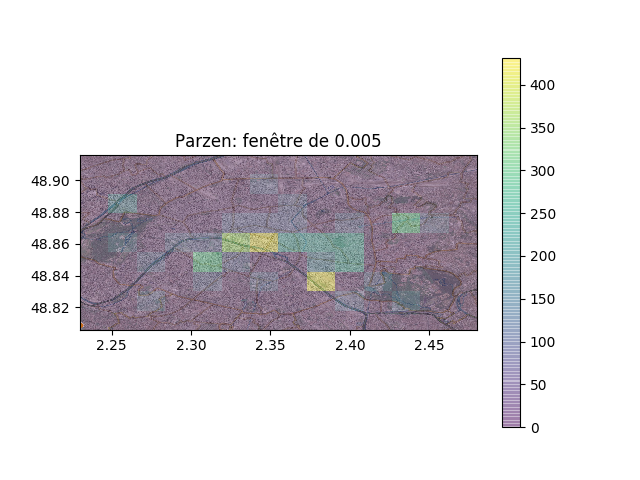
\includegraphics[scale=0.5]{Parzen0005.png}
\label{f1_trajectoire}
\end{minipage}\hfill
\begin{minipage}{0.45\textwidth}
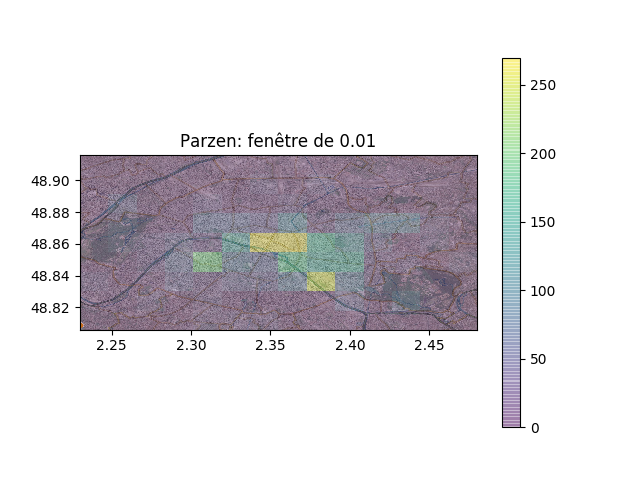
\includegraphics[scale=0.5]{Parzen001.png}
\label{f2_trajectoire}
\end{minipage}
\end{center}
\end{figure}

\begin{figure}[ht!]
\begin{center}
\begin{minipage}{0.45\textwidth}
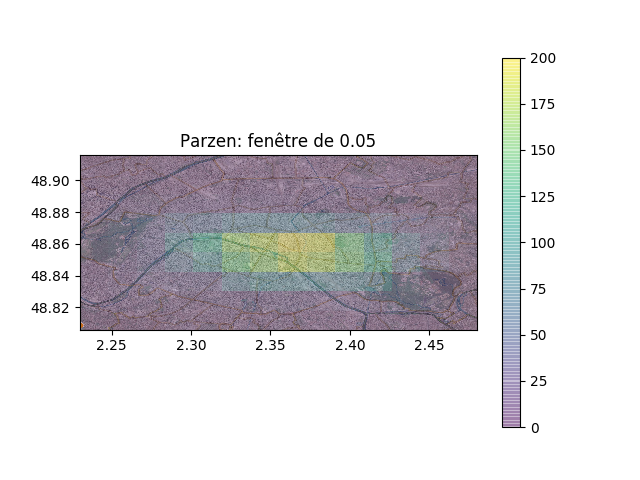
\includegraphics[scale=0.5]{Parzen005.png}
\label{f1_trajectoire}
\end{minipage}\hfill
\begin{minipage}{0.45\textwidth}
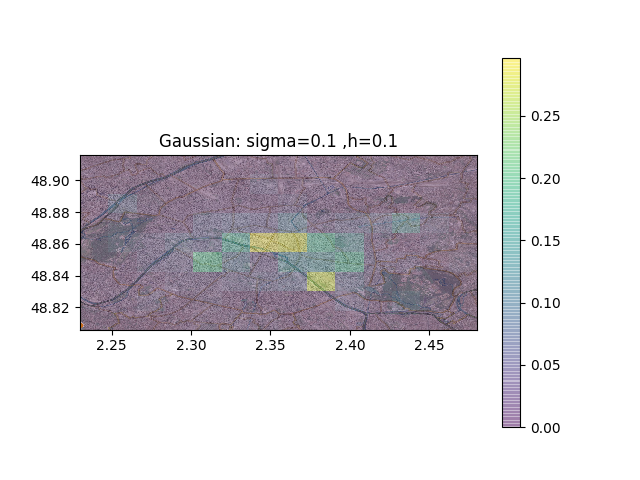
\includegraphics[scale=0.5]{Gaussian01.png}
\label{f2_trajectoire}
\end{minipage}
\end{center}
\end{figure}

\begin{figure}[ht!]
\begin{center}
\begin{minipage}{0.45\textwidth}
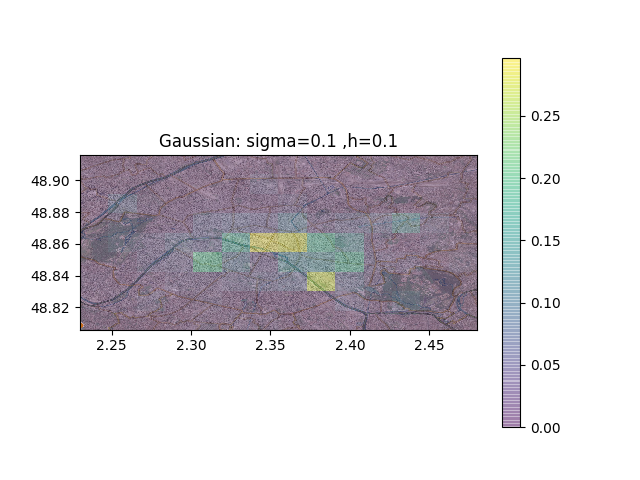
\includegraphics[scale=0.5]{Gaussian01.png}
\label{f1_trajectoire}
\end{minipage}\hfill
\begin{minipage}{0.45\textwidth}
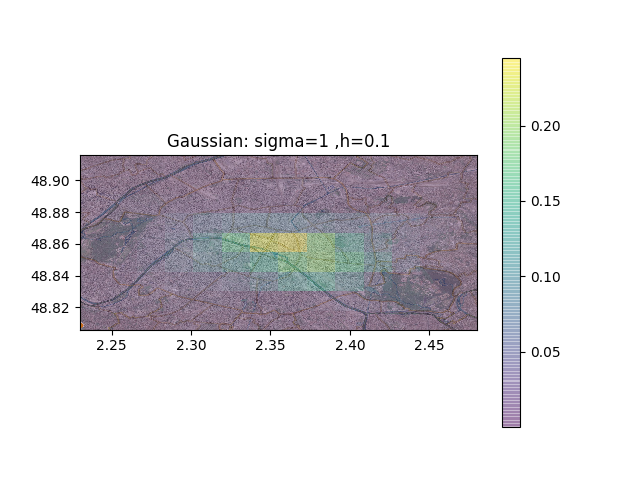
\includegraphics[scale=0.5]{Gaussian10.png}
\label{f2_trajectoire}
\end{minipage}
\end{center}
\end{figure}

Pour les méthodes à noyaux, le paramètre h est pertinent uniquement pour le cas de la fenêtre de Parzen. Pour le noyau Gaussien c'est l'écart type qui s'est avéré discriminant. On voit que pour la fenêtre de Parzen, il faut environ h égal à 0.01 pour avoir une estimation correcte, et que passé 0.05 notre densité commence à devenir floue. Le même constat se fait pour un noyau gaussien : il faut un écart-type aux alentours de 0.1.

\subsection*{Choix automatique des meilleurs paramètres}

Pour trouver automatiquement les meilleurs paramètres on a effectué un grid search avec des échelles logarithmiques.

\subsection*{Estimation de la qualité du modèle}

Pour estimer graphiquement la qualité du modèle on peut générer un échantillon suivant la densité obtenue et voir si cela correspond aux données.

\section*{TME 3 - Descente de gradient}

L'ensemble des implémentations de ce qui est décrit dans la suite sont codées dans le fichier \verb!TME3/tme3-etu.py!. A noter que celui-ci s'appuie entre autres sur \verb!arftools.py!, que l'on utilise pour sa fonction \verb!gen_arti! pour tester notre modèle.

\subsection*{Optimisation de fonctions}

On étudie dans cette partie les trois fonctions $f_1(x) = x \cos(x)$, $f_2(x) = x^2 - \log(x)$ et $f_3(x_1, x_2) = 100(x_2-x_1^2)^2 + (1-x_1)^2$.

L'algorithme de descente de gradient est testé sur ces trois fonctions. On visualise ce-dessous les trajectoires d'optimisation sur celles-ci. Pour $f_1$ et $f_2$, cet affichage est logiquement en 2D (Figures \ref{f1_trajectoire} et \ref{f2_trajectoire}). L'algorithme de descente de gradient est initialisé à $x=5$, avec un pas de 0.1 et 30 itérations. La fonction $f_3$ est quant à elle affichée en 3D. L'algorithme est initialisée à $(x_1, x_2)=(5, 5)$ avec un pas de 0.001 et 20 itérations (Figure \ref{f3_trajectoire}).

\begin{figure}[ht!]
\begin{center}
\begin{minipage}{0.45\textwidth}
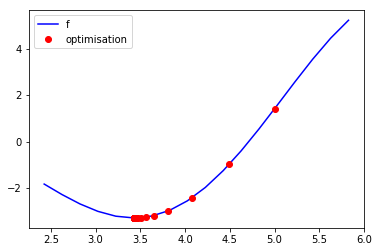
\includegraphics[scale=0.5]{f1_trajectoire.png}
\caption{Trajectoire d'optimisation de $f_1$}
\label{f1_trajectoire}
\end{minipage}\hfill
\begin{minipage}{0.45\textwidth}
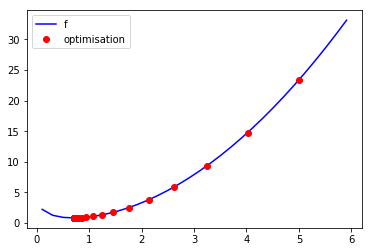
\includegraphics[scale=0.5]{f2_trajectoire.png}
\caption{Trajectoire d'optimisation de $f_2$}
\label{f2_trajectoire}
\end{minipage}
\end{center}
\end{figure}

\begin{figure}[ht!]
\begin{center}
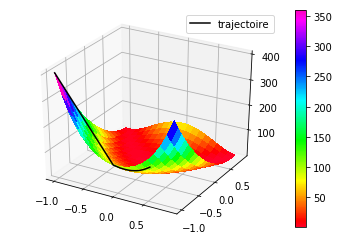
\includegraphics[scale=0.5]{f3_trajectoire.png}
\caption{Trajectoire d'optimisation de $f_3$}
\label{f3_trajectoire}
\end{center}
\end{figure}

Les Figures \ref{f1_optim_grad}, \ref{f2_optim_grad} et \ref{f3_optim_grad} montrent, pour chacune des trois fonction, la valeur de l'estimation de son optimumainsi que son gradient, en fonction du nombre d'itérations. On constate que pour toutes les trois, l'optimum est obtenu assez rapidement (en une dizaine d'itérations). Les réglages sont identiques à ceux des figures précédentes.

\begin{figure}[ht!]
\begin{center}
\begin{minipage}{0.45\textwidth}
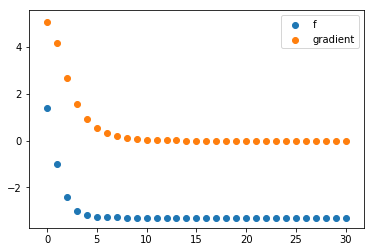
\includegraphics[scale=0.5]{f1_optim_grad.png}
\caption{Valeur de $f_1$ et de son gradient}
\label{f1_optim_grad}
\end{minipage}\hfill
\begin{minipage}{0.45\textwidth}
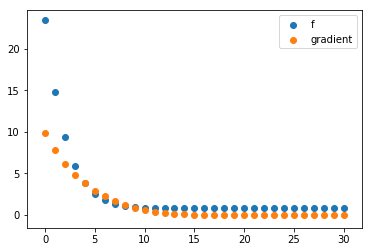
\includegraphics[scale=0.5]{f2_optim_grad.png}
\caption{Valeur de $f_2$ et de son gradient}
\label{f2_optim_grad}
\end{minipage}
\end{center}
\end{figure}

\begin{figure}[ht!]
\begin{center}
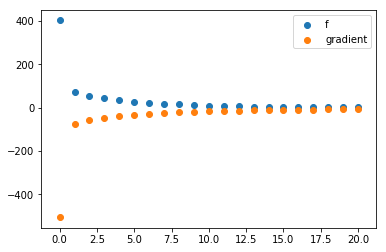
\includegraphics[scale=0.5]{f3_optim_grad.png}
\caption{Valeur de $f_3$ et de son gradient (moyenne sur $x_1$ et $x_2$)}
\label{f3_optim_grad}
\end{center}
\end{figure}

On propose enfin d'afficher les courbes de log distance entre la valeur estimée de la fonction et la valeur optimale globale, en fonction de l'itération. Les résultats sont proposés dans les Figures \ref{f1_logdist}, \ref{f2_logdist} et \ref{f3_logdist}. On semble constater que $f_1$ et $f_2$ ont une log distance proportionnelle en fonction du nombre d'itération, c'est à dire que la distance diminue exponentiellement. La forme de la fonction de $f_3$ est moins facilement interprétatble, et semble "accélérer sa diminution" avec l'augmentation de l'itération (entre 40 et 50).

\begin{figure}[ht!]
\begin{center}
\begin{minipage}{0.45\textwidth}
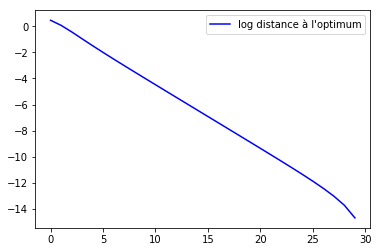
\includegraphics[scale=0.5]{f1_logdist.png}
\caption{Log distance de $f_1$ à l'optimum}
\label{f1_logdist}
\end{minipage}\hfill
\begin{minipage}{0.45\textwidth}
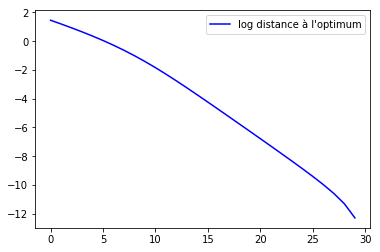
\includegraphics[scale=0.5]{f2_logdist.png}
\caption{Log distance de $f_2$ à l'optimum}
\label{f2_logdist}
\end{minipage}
\end{center}
\end{figure}

\begin{figure}[ht!]
\begin{center}
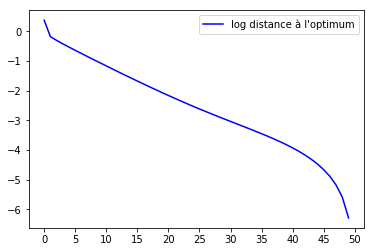
\includegraphics[scale=0.5]{f3_logdist.png}
\caption{Log distance de $f_3$ à l'optimum}
\label{f3_logdist}
\end{center}
\end{figure}

\subsection*{Régression logistique}

La classe correspondant au classifieur basé sur la régression logistique est nommé \verb!Learner! dans notre implémentation sous Python. Il dispose d'une méthode d'initialisation, des méthodes \verb!fit!, \verb!predict! et \verb!score! comme définies dans l'énoncé, ainsi que des méthodes \verb!loss! qui calcule l'erreur des associée à ce modèle aux données passées en entrée, et d'une méthode \verb!grad_loss! qui fournit le gradient de cette fonction d'erreur.

On commence par tester ce classifieur sur les données générées artificiellement grâce à la fonction \verb!gen_arti! empruntée aux outils du TME4 : celui-ci se révèle très performant sur ces données, avec une erreur de $8\%$ en entrainement et $9\%$ en test (voir Figure \ref{mse_genarti}).

\begin{figure}[ht!]
\begin{center}
\begin{minipage}{0.45\textwidth}
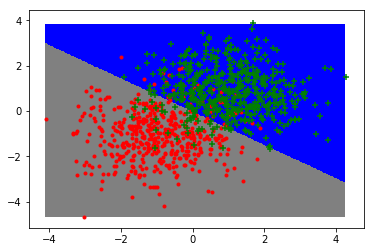
\includegraphics[scale=0.5]{mse_genarti.png}
\caption{Frontière de décision de la régression logistique}
\label{mse_genarti}
\end{minipage}\hfill
\begin{minipage}{0.45\textwidth}
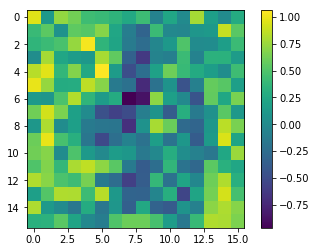
\includegraphics[scale=0.5]{weights_usps.png}
\caption{Affichage graphique des 256 poids du classifieur, sous forme de matrice $16 \times 16$}
\label{weights_usps}
\end{minipage}
\end{center}
\end{figure}

On teste ensuite notre classifieur sur les données USPS. Celui-ci s'avère remarquablement performant : par exemple sur la reconnaissance des "6" contre les "9", il obtient une erreur de 0.0\% en entrainement et 0.1\% en test. Pour la reconnaissance des "1" contre toutes les autres classes, il obtient un score de classification incorrecte de 1.4\% en entrainement et 2.5\% en test.

On propose ci-dessous un affichage graphique du vecteur de poids déterminé par l'algorithme pour la classification 6 vs. 9. Celui-ci étant de taille 256, on l'a reformaté sous forme d'une matrice $16 \times 16$ pour retrouver les dimension des images. Cet affichage est proposé en Figure \ref{weights_usps}. Pour cette classification, nous avons transformé les labels "6" en $-1$ et les labels "9" en $+1$ (après avoir isolé les seules images de 6 et de 9). On pourrait donc s'attendre à trouver des poids faibles sur les pixels traçant un 6, et des poids forts pour ceux traçants un 9. La Figure \ref{weights_usps} ne semble pas montrer de tels motifs, sûrement à cause du chevauchements des formes "6" et "9".

\section*{TME 4 et 5 - Perceptron}

L'ensemble des implémentations de ce qui est décrit dans la suite sont codées dans le fichier \verb!TME4/tme4-etu.py!. A noter que celui-ci s'appuie entre autres sur \verb!arftools.py!.

\subsection*{Implémentation}

La bonne implémentation des fonctions de coût MSE et Hinge ainsi que de leur gradient respectif est bien vérifiée par l'affichage de leurs isocontours (voir Figures \ref{isocontour_mse} et \ref{isocontour_hinge}).

\begin{figure}[ht!]
\begin{center}
\begin{minipage}{0.45\textwidth}
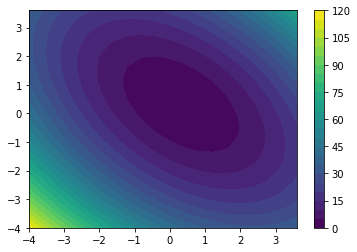
\includegraphics[scale=0.5]{isocontour_mse.png}
\caption{Isocontours de la fonction d'erreur MSE}
\label{isocontour_mse}
\end{minipage}\hfill
\begin{minipage}{0.45\textwidth}
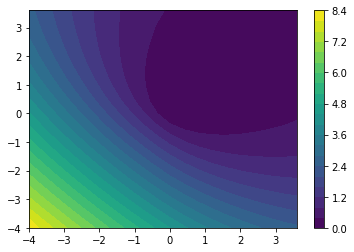
\includegraphics[scale=0.5]{isocontour_hinge.png}
\caption{Isocontours de la fonction d'erreur Hinge}
\label{isocontour_hinge}
\end{minipage}
\end{center}
\end{figure}

On vérifie également bien que l'implémentation de \verb!Lineaire! est correcte grâce au données de \verb!gen_arti! : comme régression linéaire elle obtient une classification incorrecte de $14.5\%$ en entrainement et $14.3\%$ en test (voir Figure \ref{frontiere_mse}), et comme perceptron $9.6\%$ en entrainement et $8.5\%$ en test (Figure \ref{frontiere_hinge}).

\begin{figure}[ht!]
\begin{center}
\begin{minipage}{0.45\textwidth}
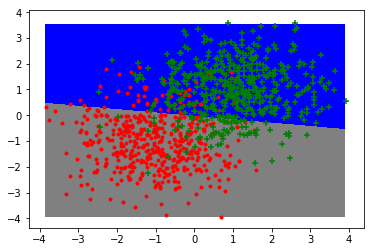
\includegraphics[scale=0.5]{frontiere_mse.png}
\caption{Frontière de la régression linéaire}
\label{frontiere_mse}
\end{minipage}\hfill
\begin{minipage}{0.45\textwidth}
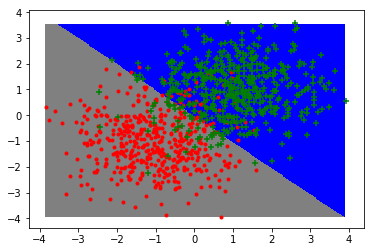
\includegraphics[scale=0.5]{frontiere_hinge.png}
\caption{Frontière du perceptron}
\label{frontiere_hinge}
\end{minipage}
\end{center}
\end{figure}

On propose également d'afficher la trajectoire d'optimisation sur la surface d'isocontour des fonctions d'erreur pour vérifier la bonne convergence. Celle-ci semble bonne dans les Figures \ref{trajectoire_mse} et \ref{trajectoire_hinge}.

\begin{figure}[ht!]
\begin{center}
\begin{minipage}{0.45\textwidth}
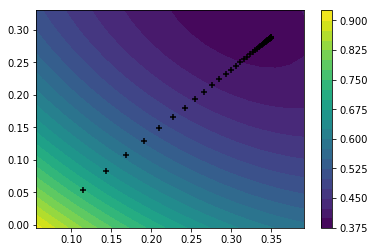
\includegraphics[scale=0.5]{trajectoire_mse.png}
\caption{Trajectoire d'optimisation pour la fonction MSE}
\label{trajectoire_mse}
\end{minipage}\hfill
\begin{minipage}{0.45\textwidth}
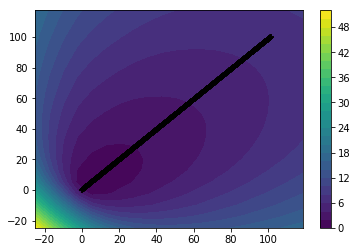
\includegraphics[scale=0.5]{trajectoire_hinge.png}
\caption{Trajectoire d'optimisation pour la fonction Hinge}
\label{trajectoire_hinge}
\end{minipage}
\end{center}
\end{figure}

On implémente également dans notre classe \verb!Lineaire! une bossibilité d'ajouter un biais : il suffif pour cela de fixer la variable \verb!self.bias! sur True. L'ajout de ce biais permet (étonnamment) d'obtenir de moins bons résultats pour la régression linéaire ($11.5\%$ d'erreur en test) mais quelques peu meilleurs pour le perceptron ($8.2\%$). Les frontières de décisions sont affichées dans les Figures \ref{frontiere_mse_biais} et \ref{frontiere_hinge_biais}.

\begin{figure}[ht!]
\begin{center}
\begin{minipage}{0.45\textwidth}
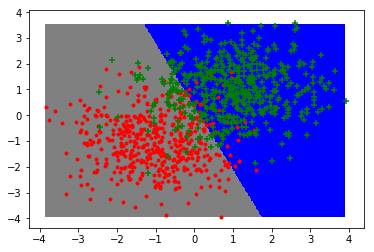
\includegraphics[scale=0.5]{frontiere_mse_biais.png}
\caption{Frontière de décision de la régression linéaire avec biais}
\label{frontiere_mse_biais}
\end{minipage}\hfill
\begin{minipage}{0.45\textwidth}
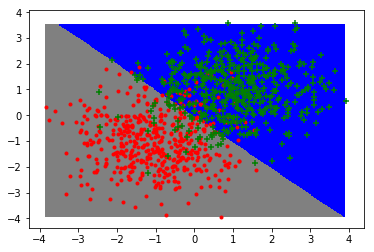
\includegraphics[scale=0.5]{frontiere_hinge_biais.png}
\caption{Frontière de décision du perceptron avec biais}
\label{frontiere_hinge_biais}
\end{minipage}
\end{center}
\end{figure}

\subsection*{Données USPS}

On commence par étudier la capacité de notre perceptron à distinguer les deux classes "6" et "9", comme on l'avait fait pour la régression linéaire au TME précédent. Comme pour cette dernière, le perceptron s'avère très efficace : son taux d'erreur en entrainement est de $0.2\%$, et de $0.7\%$. On affiche dans la Figure \ref{weights_mse_6v9} le vecteur de 256 poids sous forme d'une matrice $16 \times 16$ de manière similaire à ce que nous avions fait dans le TME3. Cependant le résultat est cette fois-ci bien plus intéressant : on discerne clairement que les poids correspondant aux pixels placés sur le tracé du "6" (encodé en $-1$) sont fortement négatifs, tandis que ceux placés sur le tracés d'un "9" ($+1$) sont fortement positifs. Les autres sont proches de 0.

On réitère l'entrainement en tentant cette fois-ci de faire discerner le "6" de toutes les autres classes. les résultats sont encore bons, avec un taux d'erreur de $8.4\%$ en entrainement et $9.1\%$ en test. L'affichage du vecteur de poids (Figure \ref{weights_mse_6vAll}) nous permet de constater cette fois-ci que tous les poids sont négatifs (on a encodé $+1$ si c'est un "6", $-1$ sinon) : on peut donc dire que le classifieurs cherche à reconnaitre tous les autres chiffres que le 6, comme le montre l'activation des poids sur ce qui semble être le tracé d'un "3" ou d'un "8".

\begin{figure}[ht!]
\begin{center}
\begin{minipage}{0.45\textwidth}
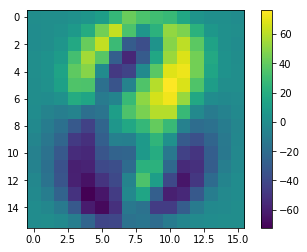
\includegraphics[scale=0.5]{weights_mse_6v9.png}
\caption{Vecteur des 256 poids (sous forme $16 \times 16$) du perceptron pour 6 vs. 9}
\label{weights_mse_6v9}
\end{minipage}\hfill
\begin{minipage}{0.45\textwidth}
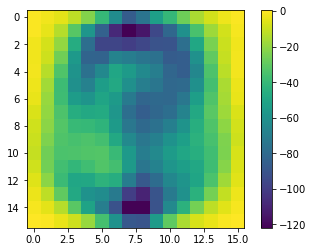
\includegraphics[scale=0.5]{weights_mse_6vAll.png}
\caption{Vecteur des 256 poids (sous forme $16 \times 16$) du perceptron pour 6 vs. le reste}
\label{weights_mse_6vAll}
\end{minipage}
\end{center}
\end{figure}

Les courbes d'apprentissage (erreur en fonction du nombre d'itération), proposée pour chacun de ces deux problèmes (Figures \ref{learning_curve_6v9} et \ref{learning_curve_6vAll}) nous montre qu'il n'y a pas de sur-apprentissage dans ce cas-ci

\begin{figure}[ht!]
\begin{center}
\begin{minipage}{0.45\textwidth}
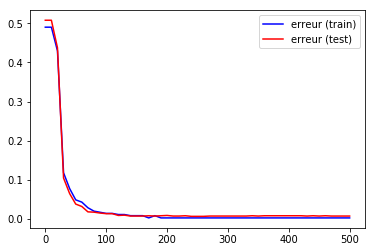
\includegraphics[scale=0.5]{learning_curve_6v9.png}
\caption{Courbe d'apprentissage du perceptron pour 6 vs. 9}
\label{learning_curve_6v9}
\end{minipage}\hfill
\begin{minipage}{0.45\textwidth}
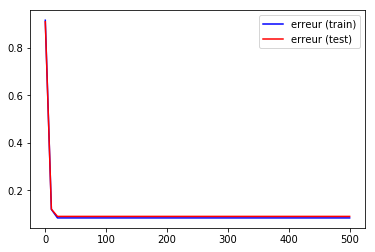
\includegraphics[scale=0.5]{learning_curve_6vAll.png}
\caption{Courbe d'apprentissage du perceptron pour 6 vs. le reste}
\label{learning_curve_6vAll}
\end{minipage}
\end{center}
\end{figure}

\subsection*{Données 2D et projection}

On cherche maintenant à ajouter des projections pour améliorer l'expressivité de notre perceptron. On commence par lui ajouter une projection gaussienne (en fixant, dans la classe \verb!Lineaire!, la valeur \verb!projec! sur "gauss"), en utilisant comme base un ensemble de 100 exemples de la base d'exemples tirés au hasard (et passés en valeur de \verb!self.base!). Le taux d'erreur n'est pas vraiment amélioré : il est de $9.5\%$ en apprentissage et $10.3\%$ en test. La Figure \ref{frontiere_hinge_gauss} nous montre que la frontière n'est plus linéaire mais semble "overfitter" quelques-uns des points proches de la séparation.

Nous avons également appliqué une projection polynomiale sur les données 2D. On n'obtient pas là non plus de résultats significativement meilleurs : le taux d'erreur en apprentissage est de $9.5\%$, et $8.6\%$ en test. Il n'y a donc cette fois-ci sûrement pas de surapprentissage, mais la forme conique de la courbe n'aide pas à séparer les poids des deux gaussiennes qui se chevauchent. La frontière avec cette projection est affichée dans la Figure \ref{frontiere_hinge_poly}.

\begin{figure}[ht!]
\begin{center}
\begin{minipage}{0.45\textwidth}
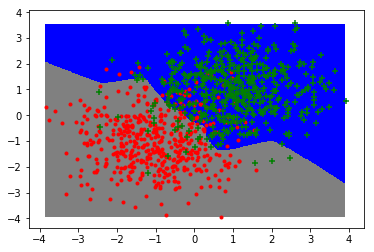
\includegraphics[scale=0.5]{frontiere_hinge_gauss.png}
\caption{Frontière du perceptron avec projection gaussienne}
\label{frontiere_hinge_gauss}
\end{minipage}\hfill
\begin{minipage}{0.45\textwidth}
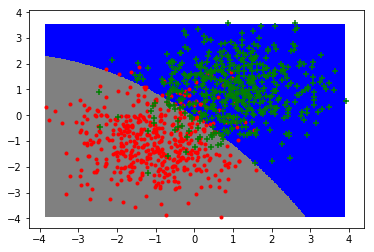
\includegraphics[scale=0.5]{frontiere_hinge_poly.png}
\caption{Frontière du perceptron avec projection polynomiale}
\label{frontiere_hinge_poly}
\end{minipage}
\end{center}
\end{figure}

\section*{TME 6 - SVM et Noyaux}

Dans cette partie nous cherchons à faire de la classification sur les mêmes données qu'au TME5, mais en utilisant les Support Vector Machines (SVM). Notre outil principal aura été \verb!scikit-learn!. Nous avons testé quatre kernels distincts : kernel linéaire, polynomial, rbf et sigmoid. 

\begin{figure}[ht!]
\begin{center}
\begin{minipage}{0.45\textwidth}
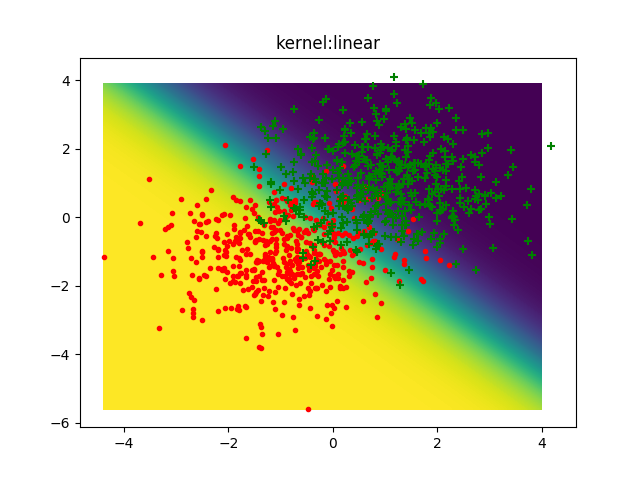
\includegraphics[scale=0.5]{linear.png}
\label{f1_logdist}
\end{minipage}\hfill
\begin{minipage}{0.45\textwidth}
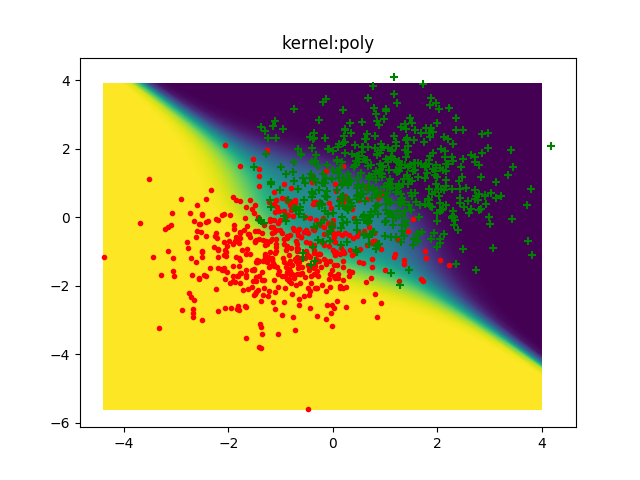
\includegraphics[scale=0.5]{poly.png}
\label{f2_logdist}
\end{minipage}
\end{center}
\end{figure}

\begin{figure}[ht!]
\begin{center}
\begin{minipage}{0.45\textwidth}
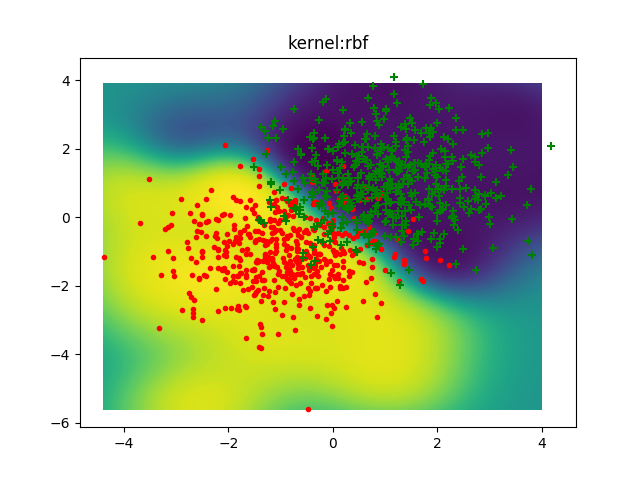
\includegraphics[scale=0.5]{rbf.png}
\label{f1_logdist}
\end{minipage}\hfill
\begin{minipage}{0.45\textwidth}
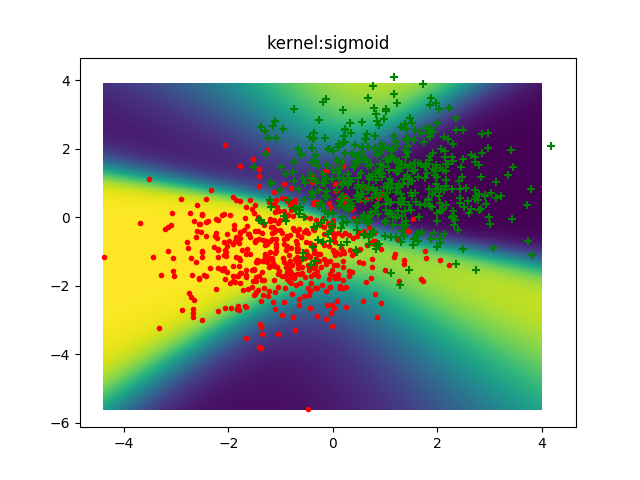
\includegraphics[scale=0.5]{sigmoid.png}
\label{f2_logdist}
\end{minipage}
\end{center}
\end{figure}

On voit que les noyaux linéaires et polynomiaux ont des comportements similaires, à cela près que le kernel polynomial est moins certain pour les points à la frontière. Le kernel qui sépare le mieux est rbf, et sigmoid est complètement à côté de la plaque.

\end{document}

